\documentclass[]{article}

% Use utf-8 encoding for foreign characters
\usepackage[utf8]{inputenc}

% Setup for fullpage use
\usepackage{fullpage}
\usepackage{graphicx}

\usepackage[francais]{babel}

\usepackage{times}
%\usepackage{rotate}
%\usepackage{lscape}

\usepackage{color}

\usepackage{needspace}

\usepackage{float}

\newcommand{\placeholder}[1]{{\noindent \color{red}[ #1 ]}}

\begin{document}

%\frontmatter          % for the preliminaries
%\pagestyle{headings}  % switches on printing of running heads
%\mainmatter              % start of the contributions

\title{
{\Huge Maquette d'interface utilisateur}\\
Projet de Génie Logiciel\\
\smallskip
{\small Activité d'Apprentissage \textsf{S-INFO-015}}\\
}

\author{Groupe numéro: 3\\
Membres du groupe:\\
\textbf{DOM Eduardo , DHEUR Victor, AMEZIAN Aziz}\\
}


\date{Année Académique : 2017 - 2018\\
BAC 2 en Sciences Informatiques\\
\vspace{1cm}
Faculté des Sciences, Université de Mons}


%\title{Projet de Génie Logiciel\\
%Rapport de Planification\\
%Année Académique ****-****\\
%}
%\title{{\Huge Rapport de Planification}\\
%Projet de Génie Logiciel\\
%{\small
%	Unités d'Enseignement \textsf{US-B2-SCINFO-009-M}, \textsf{US-B3-SCMATH-013-M}, \textsf{US-M1-SCINFO-045-M}\\
%	Activité d'Apprentissage \textsf{S-INFO-015}
%}\\
%
%\date{Année Académique 2015-2016\\
%Bachelier en Sciences Informatiques\\
%Bloc complémentaire en Master I Informatique\\
%\vspace{1cm}
%Faculté des Sciences, Université de Mons}
%
%
%
%%\titlerunning{Rapport de planification -- \textbf{ANNEE ACADEMIQUE}}
%
%
%\authorrunning{Groupe \textbf{**} - \textbf{ANNEE D'ETUDES}} 

%\institute{\textbf{ANNEE D'ETUDES (par exemple BAC 2 INFO ou ANNEE PREPA)}\\
%Faculté des Sciences, Université de Mons\\
%\email{\{ PRENOM1.NOM1 $\mid$ PRENOM2.NOM2 \}@student.umons.ac.be}
%VOUS POUVEZ UTILISER UN AUTRE ADRESSE MAIL QUE CELUI DE L'UMONS SI VOUS LE PREFERIEZ
%}

\maketitle              % typeset the title of the contribution

\bigskip
\begin{center} \today \end{center}

\newpage
%%%%%%%%%%%%%%%%%%%%%%%%%%%%%%%%%%%%%%%%%%%%%%%%
%%%%%%%%%%%%%%%%%%%%%%%%%%%%%%%%%%%%%%%%%%%%%%%%
\section{Introduction}\label{sec:welcome}
Dans ce rapport nous allons vous présenter l'interface utilisateur que nous allons implémenter pour notre projet. Des images illustrant chaque état sont présentes dans ce document et sont aussi disponibles en annexe.

\section{Menu Principal}\label{sec:welcome}

\begin{figure}[!htb]
\begin{center}
  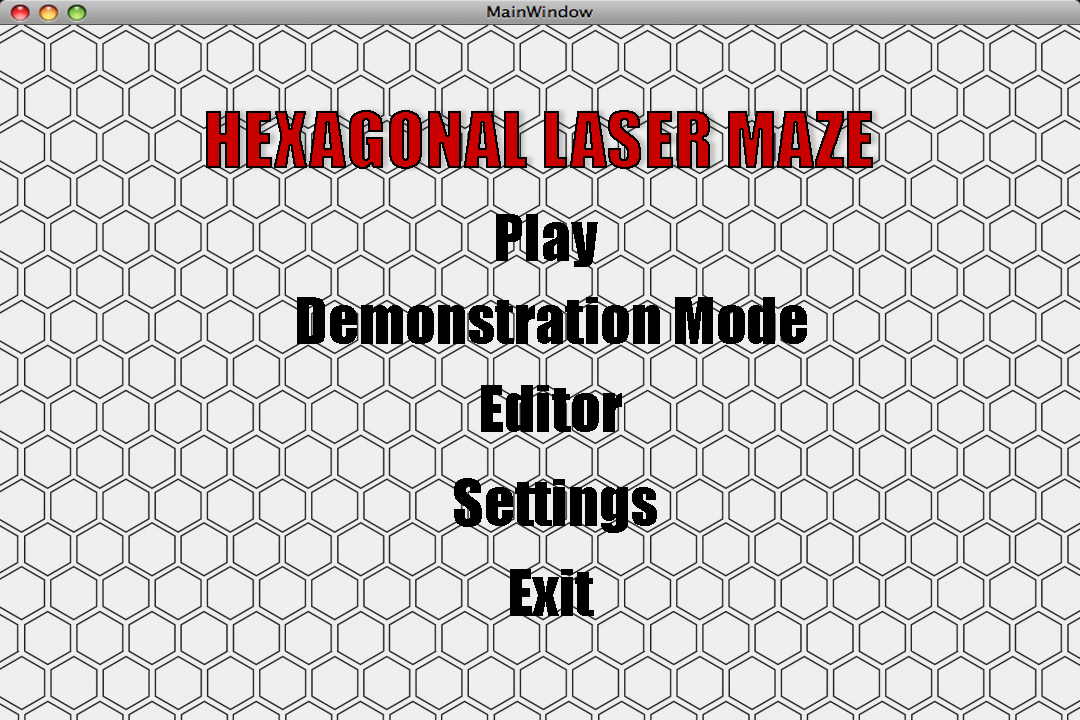
\includegraphics[width=\textwidth]{Welcome.png}
  \caption{Menu principal.}\label{fig:welcome}
\end{center}
\end{figure}

Lorsque l'utilisateur lance le jeu, la première interface que lui sera présenté sera le menu principal. Dans celui-ci, 5 boutons lui sont accessibles:
\begin{enumerate}
\item Play : Permet à l'utilisateur d'accéder à l'écran de sélection de niveau.
\item Automatic Mode : Permet à l'utilisateur d'accéder au mode de jeu automatique.
\item Editor : Permet à l'utilisateur d'accéder à l'éditeur de niveaux.
\item Settings : Permet à l'utilisateur d'accéder aux options du jeu.
\item Quit : Permet à l'utilisateur de quitter le jeu.
\end{enumerate}

\newpage
\section{Sélection de niveaux}\label{sec:select}

\begin{figure}[!htb]
\begin{center}
  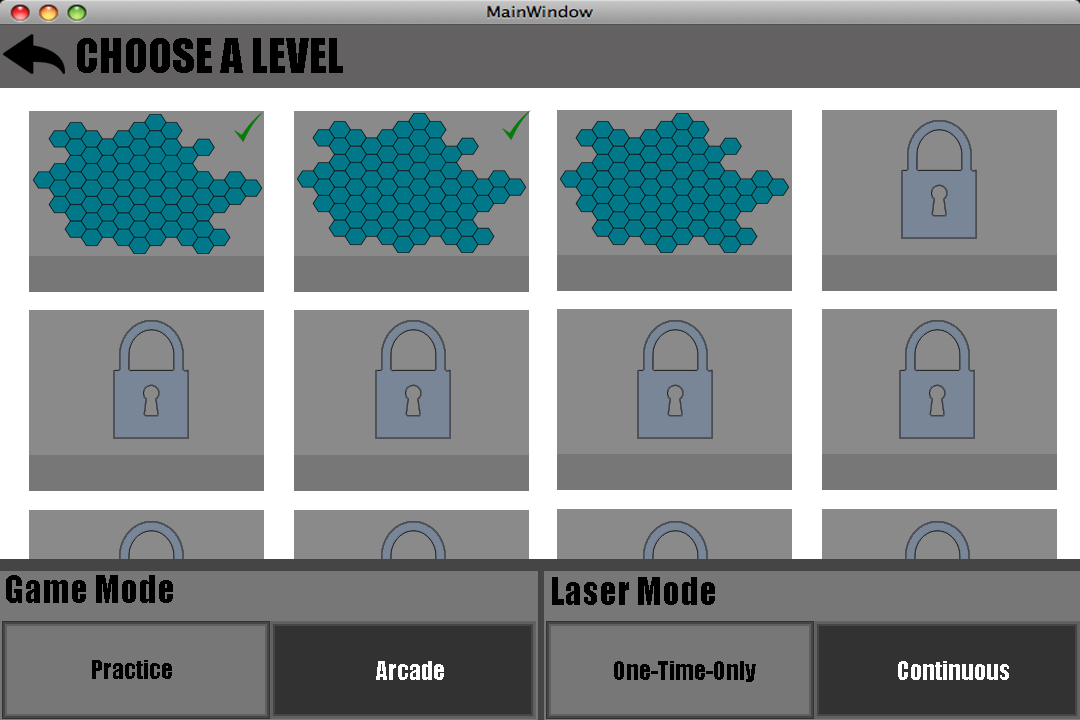
\includegraphics[width=\textwidth]{Select.png}
  \caption{Sélection de niveaux.}\label{fig:select}
\end{center}
\end{figure}

Dans le menu de sélection de niveaux, de nombreux niveaux sont offerts à l'utilisateur sous la forme de rectangles donnant un aperçu du niveau. Un "check" vert est affiché si le niveau a déja été résolu et le nom du niveau est indiqué en bas du rectangle. L'utilisateur peut sélectionner un niveau en cliquant sur le rectangle correspondant. Il peut changer les options de la partie dans le menu inférieur. Finalement, il a la possibilité de revenir au menu principal grâce à la flèche située dans le coin supérieur gauche.

\newpage
\section{Partie}\label{sec:game}
\subsection{Etat initial }\label{sec:game1}
\begin{figure}[!htb]
\begin{center}
  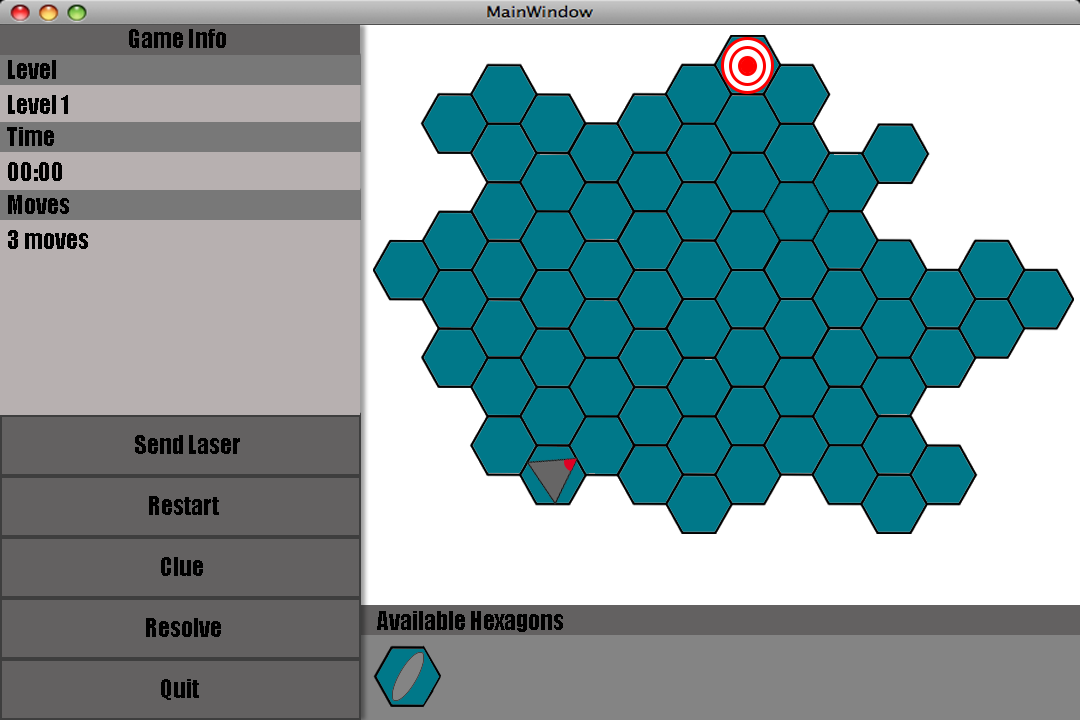
\includegraphics[width=\textwidth]{Game1.png}
  \caption{Etat initial d'une partie.}\label{fig:game1}
\end{center}
\end{figure}

Lorsque la partie commence, l'interface est divisée en plusieurs régions :
\begin{enumerate}
\item Dans la région supérieure droite, on retrouve le plateau de jeu avec les éléments non déplaçables du niveau.
\item Dans la région inférieure droite, on retrouve les éléments dont l'utilisateur dispose pour résoudre le niveau.
\item A droite, on retrouve des informations sur la partie ainsi que certains boutons :
\begin{enumerate}
\item Send Laser : Déclenche le laser (ce bouton n'est présent que dans le mode "one-time only laser").
\item Restart : Permet de recommencer le niveau.
\item Clue : Permet d'obtenir un indice sur la résolution du niveau (ce bouton est seulement disponible si l'extension "Level Checker" est activée).
\item Resolve : Permet d'obtenir le solution du niveau (ce bouton est seulement disponible si l'extension "Level Checker" est activée).
\item Quit : Permet de revenir à la sélection de niveaux.
\end{enumerate}
\end{enumerate}
\newpage 
\subsection{Déplacement d'élèments }\label{sec:game2}
\begin{figure}[!htb]
\begin{center}
  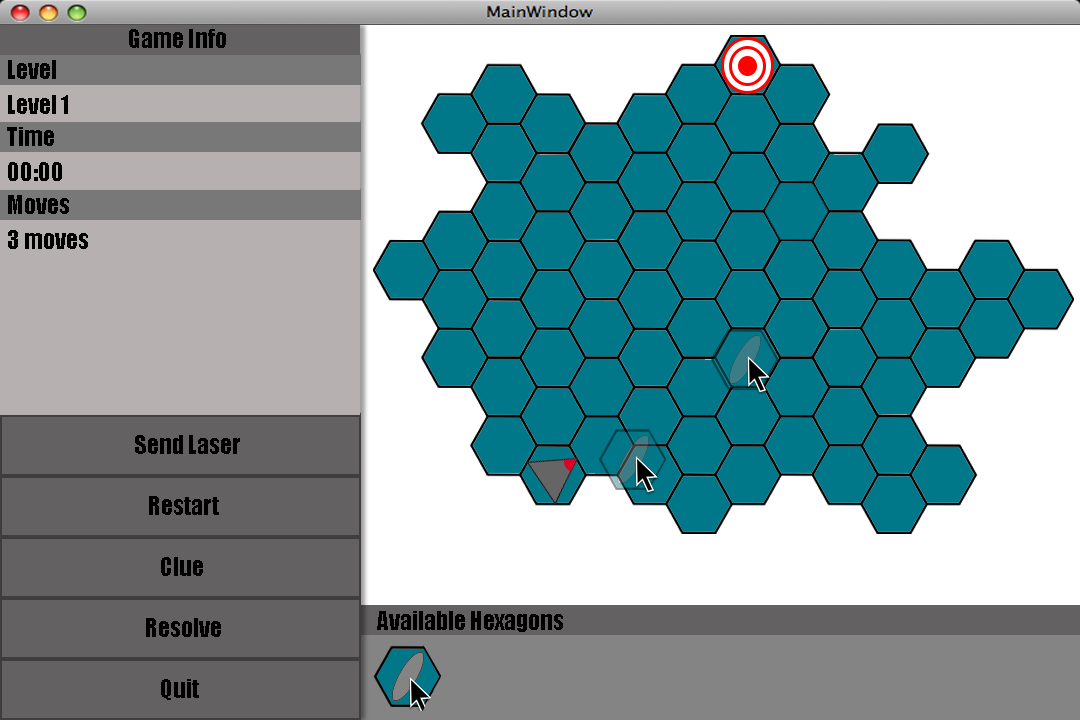
\includegraphics[width=\textwidth]{Game2.png}
  \caption{Déplacement d'un élément.}\label{fig:game2}
\end{center}
\end{figure}
L'utilisateur a la possibilité de deplacer des éléments entre le plateau de jeu et la zone "Available Hexagons" en glissant l'élèment vers sa nouvelle position.
Il peut aussi deplacer des éléments à l'intérieur du plateau de la même façon si l'élément est deplaçable.
\newpage
\subsection{Rotation d'élèments }\label{sec:game3}
\begin{figure}[!htb]
\begin{center}
  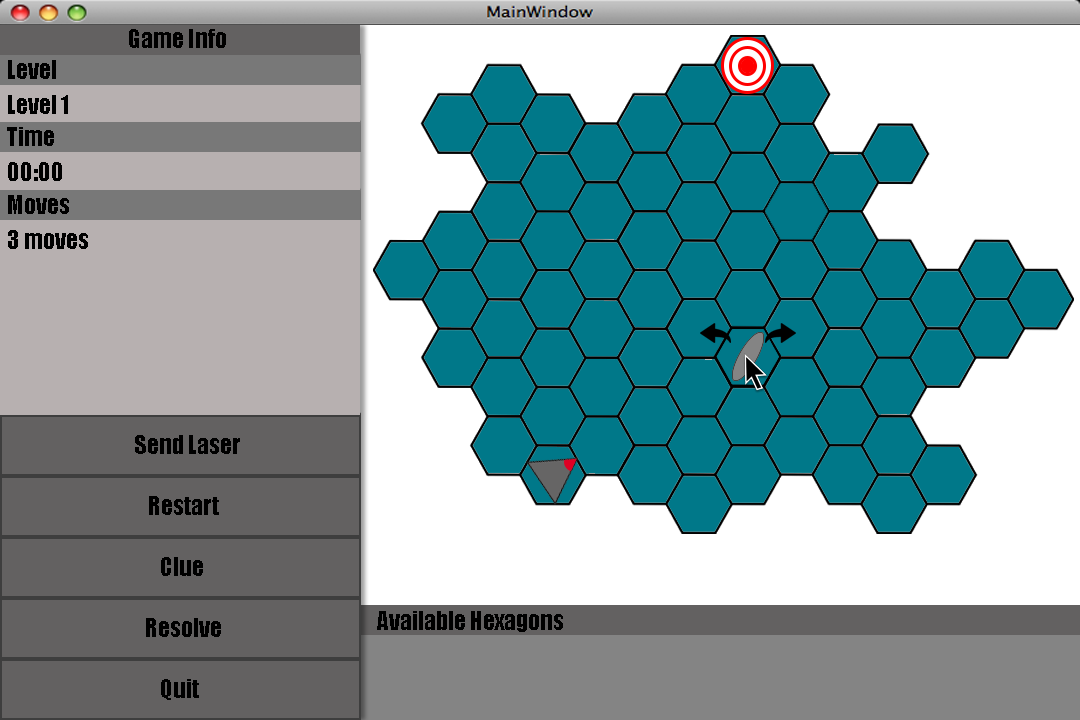
\includegraphics[width=\textwidth]{Game3.png}
  \caption{Changement de la rotation d'un élèment.}\label{fig:game3}
\end{center}
\end{figure}
Lorsque l'utilisateur fait un simple clic sur un élément sur le plateau, si celui-ci peut changer d'orientation, des flèches permettant la rotation apparaissent.
\newpage

\subsection{Lancement du laser }\label{sec:game5}
\begin{figure}[!htb]
\begin{center}
  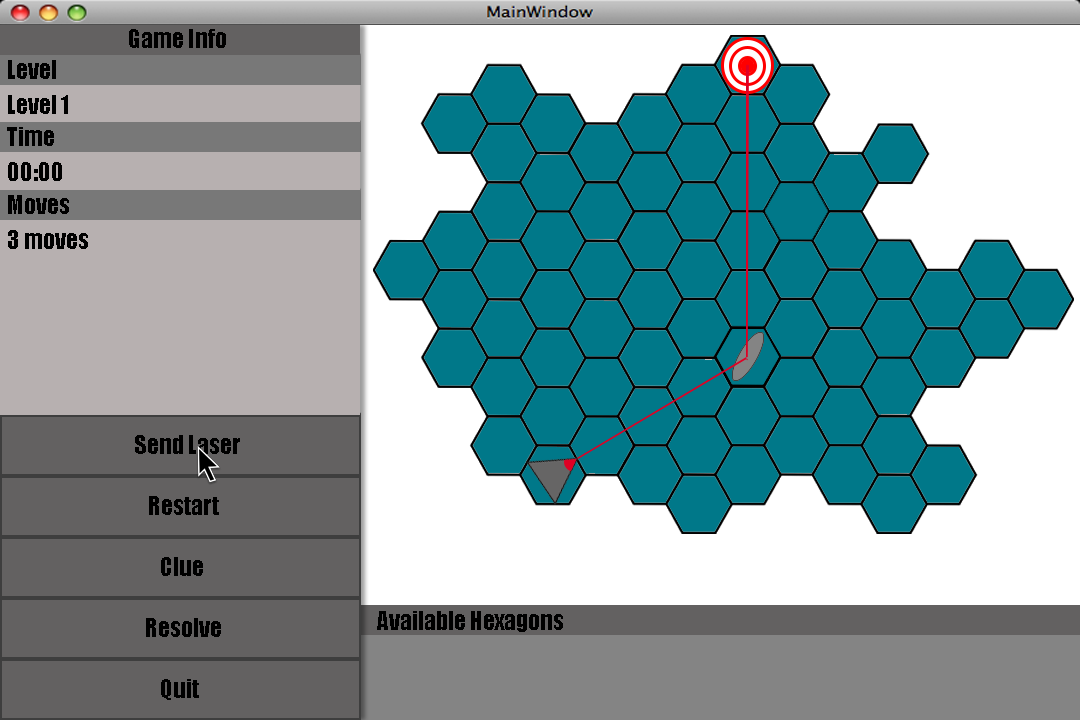
\includegraphics[width=\textwidth]{Game5.png}
  \caption{Lancement du laser.}\label{fig:game5}
\end{center}
\end{figure}
Lorsque l'utilisateur clique sur le bouton "Send Laser"(ou constamment si le mode "Continuous Laser" est activé), les lasers sont dessinés à partir des sources.
\newpage

\subsection{Fin de partie}\label{sec:game4}
\begin{figure}[!htb]
\begin{center}
  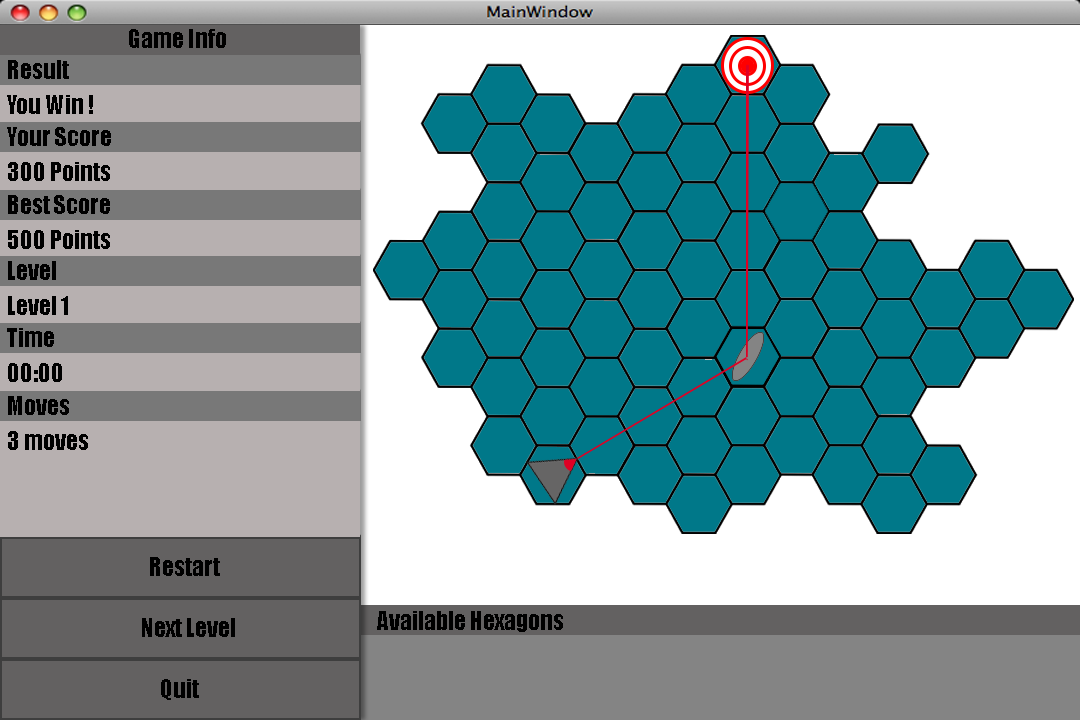
\includegraphics[width=\textwidth]{Game4.png}
  \caption{Fin de partie.}\label{fig:game4}
\end{center}
\end{figure}
Lorsque la partie se termine, la région à droite est modifiée. Certaines informations sont ajoutées :
\begin{enumerate}
\item Le résultat de la partie.
\item Le score final.
\item Le meilleur score pour ce niveau.
\end{enumerate}
En plus de cela, les boutons Send Laser, Clue et Resolve sont remplacés par un bouton Next Level qui permet de passer au niveau suivant.

\newpage
Voici quelques exemples de niveaux basiques à implémenter.
\begin{figure}[!htb]
\begin{center}
  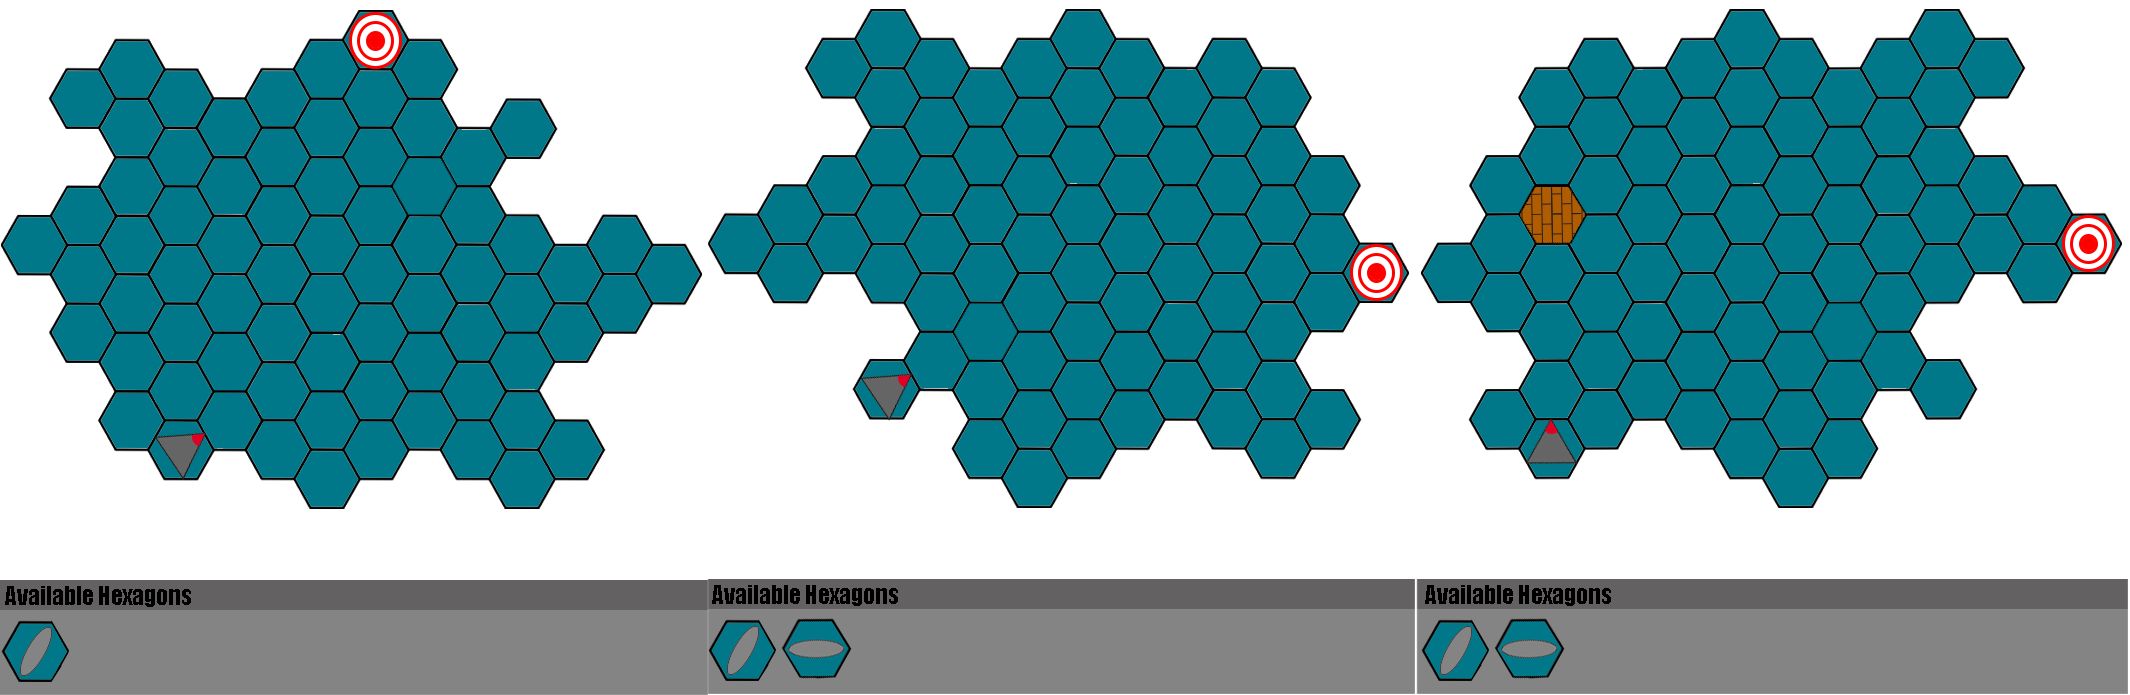
\includegraphics[width=\textwidth]{Levels.png}
  \caption{Exemples de niveau.}\label{fig:levels}
\end{center}
\end{figure}
\newpage

\section{Editeur de niveaux}\label{sec:editor}
\begin{figure}[!htb]
\begin{center}
  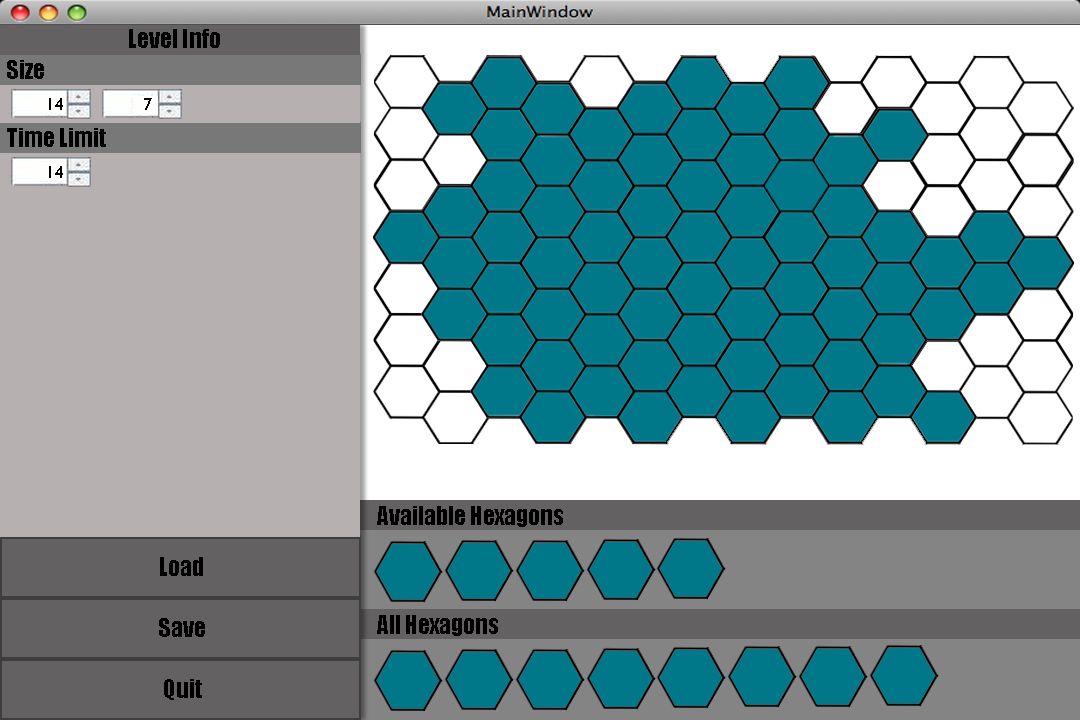
\includegraphics[width=\textwidth]{Editor.png}
  \caption{Editeur de niveaux.}\label{fig:editor}
\end{center}
\end{figure}

L'éditeur de niveaux ressemble énormément à l'interface de jeu. Dans le menu latéral, les informations sur la partie ont été remplacées par des spinners permettant de changer la taille du plateau. Nous avons aussi ajouté des boutons pour :
\begin{enumerate}
\item Tester le niveau
\item Charger un niveau
\item Sauvegarder le niveau
\end{enumerate}
Dans le menu inférieur, une deuxiéme région a été ajoutée. Dans celle-ci, tous les types d'élèments sont offerts à l'utilisateur. Il a donc la possibilité de glisser ces élèments dans la région "Available Hexagons" ou sur le plateau de jeu. Le déplacement et la rotation des éléments restent inchangés par rapport a l'interface de jeu.
\newpage
\section{Mode de jeu automatique}\label{sec:auto}
\begin{figure}[!htb]
\begin{center}
  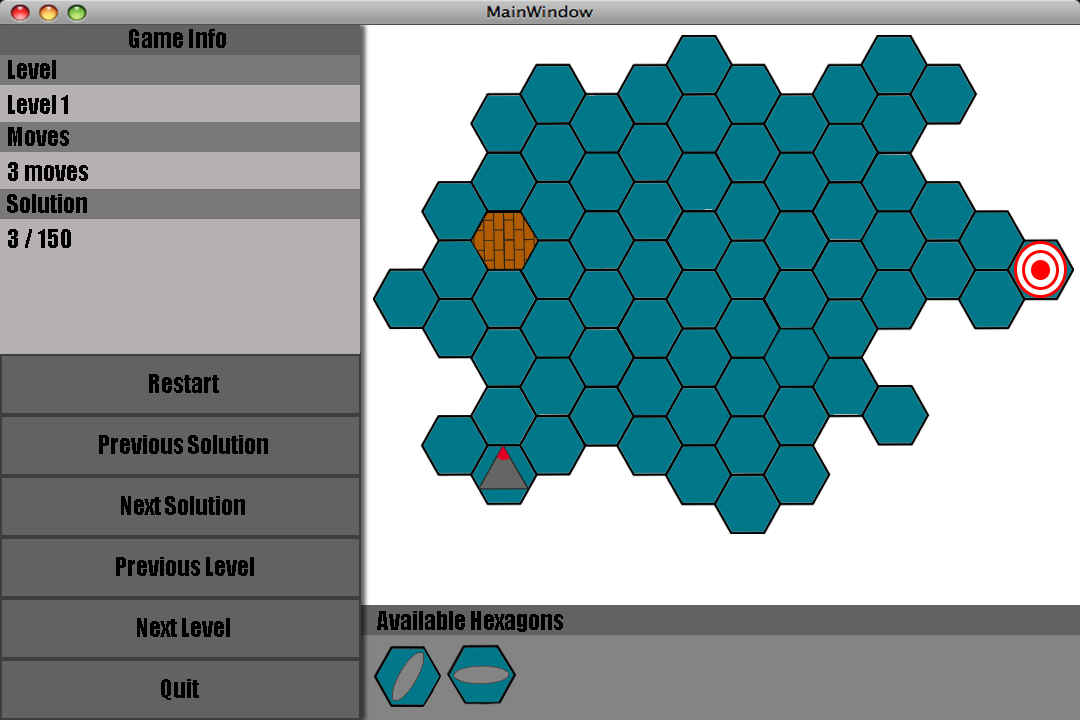
\includegraphics[width=\textwidth]{Auto.png}
  \caption{Mode de jeu automatique.}\label{fig:auto}
\end{center}
\end{figure}

Dans ce mode, le niveau est résolu automatiquement sans l'interaction de l'utilisateur.
L'interface est pratiquement identique à l'interface de jeu. La seule différence est que l'utilisateur ne peut interagir qu'avec les boutons dans le menu latéral. Avec ces boutons, il peut passer au niveau précédent ou suivant. 
\newpage
\section{Options}\label{sec:options}

\begin{figure}[!htb]
\begin{center}
  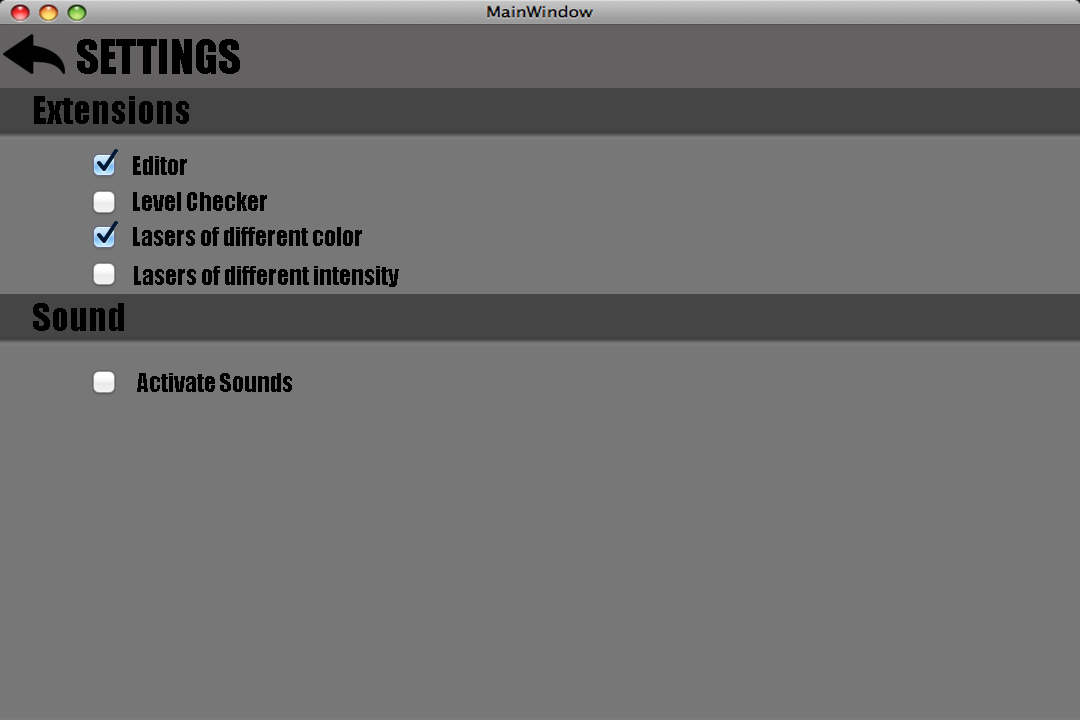
\includegraphics[width=\textwidth]{Options.png}
  \caption{Options.}\label{fig:options}
\end{center}
\end{figure}

Dans ce menu, l'utilisateur peut activer et désactiver les différentes extensions. Il a aussi la possibilité d'activer et de désactiver le son du jeu. La flèche située dans le coin supérieur gauche lui permet de revenir au menu principal.

\end{document}
